\section{Hadron spectrometry}
\label{sec:hadron-spectrometry}

The colour degree of freedom introduced in Sect.~\ref{subsec:color-experiment} completes the
quark model of the light hadrons, but the most stringent test of the model came from a
different direction: the discovery of heavy quarks and the rich spectroscopy of the bound
states they form. A heavy quark and its antiquark bind into a non-relativistic,
hydrogen-like system whose level structure can be computed from a static potential, in
close analogy to positronium. The agreement between the measured and predicted spectra of
charmonium ($c\bar c$) and bottomonium ($b\bar b$) is one of the cleanest confirmations of
the quark picture and of the short- and long-distance behaviour of the strong force. This
section follows that development. It begins with the discovery of the $J/\psi$, develops the
description of unstable states as resonances, explains the anomalously small $J/\psi$ width
through the OZI rule, introduces the quark--antiquark potential and confinement, and then
works through the quarkonium spectra. It closes with the exotic states discovered since
2003, which do not fit the simple $q\bar q$ and $qqq$ scheme.

% ============================================================
\subsection{The \texorpdfstring{$J/\psi$}{J/psi} discovery}
\label{subsec:jpsi-discovery}

In November 1974 two groups announced, almost simultaneously, the observation of an
extraordinarily narrow resonance near $3.1\,\mathrm{GeV}$---an event so consequential for
particle physics that it became known as the ``November revolution''
\cite[Ch.~8]{Amsler2018}. At the Brookhaven National Laboratory, a group led by
J.~J.~Aubert studied the reaction $p + \mathrm{Be} \to e^+e^- + \text{anything}$ and
observed a heavy particle, which they named $J$, in the $e^+e^-$ invariant-mass spectrum.
The electrons and positrons were identified by their Cherenkov radiation and time of
flight, and their momenta were measured in two magnetic spectrometers. At the same time, a
group led by J.~E.~Augustin working at the SPEAR storage ring at Stanford studied
electron--positron annihilation, $e^+e^- \to \text{hadrons},\,\mu^+\mu^-,\,e^+e^-$, and
found a narrow resonance, which they named $\psi$. The particle is now universally
denoted $J/\psi$, with a measured mass $m(J/\psi) = 3096.9\,\mathrm{MeV}$
\cite[Ch.~8]{Amsler2018}.

Two features of the SPEAR observation fixed the interpretation. First, the production
mechanism---formation directly in $e^+e^-$ annihilation through a single virtual
photon---requires the state to carry the photon's quantum numbers, $J^{PC} = 1^{--}$, just
as the $\rho$ meson does. Second, the resonance was extraordinarily narrow: the apparent
width seen at SPEAR was limited entirely by the experimental energy resolution, implying a
true width well below the few-MeV scale typical of strongly decaying hadrons. A state with
mass $3.1\,\mathrm{GeV}$ and a width of at most a few MeV is anomalous, since the available
phase space for strong decay is enormous. The resolution of this puzzle was the
identification of the $J/\psi$ as the $1\,{}^3S_1$ bound state of a new, heavy
quark--antiquark pair, $c\bar c$, carrying the new quantum number \emph{charm}, with its
narrowness explained by the OZI rule (Sect.~\ref{subsec:ozi-width})
\cite[Ch.~8]{Amsler2018}.

% ------------------------------------------------------------
% FIGURE SUGGESTION:
% Two-panel discovery figure. (left) BNL e+e- invariant-mass spectrum from
% p+Be -> e+e- + X (Aubert et al.), showing the sharp J peak near 3.1 GeV on a
% smooth background; (right) the three SPEAR excitation curves (Augustin et al.)
% for e+e- -> hadrons, e+e- -> mu+mu-, e+e- -> e+e- versus E_cms, each showing the
% psi resonance. Reproduce from the week 21 VL1 "Summary: J/psi discovery (1974)"
% slide (BNL spectrum and SPEAR scans).
% \begin{figure}[t]
%   \centering
%   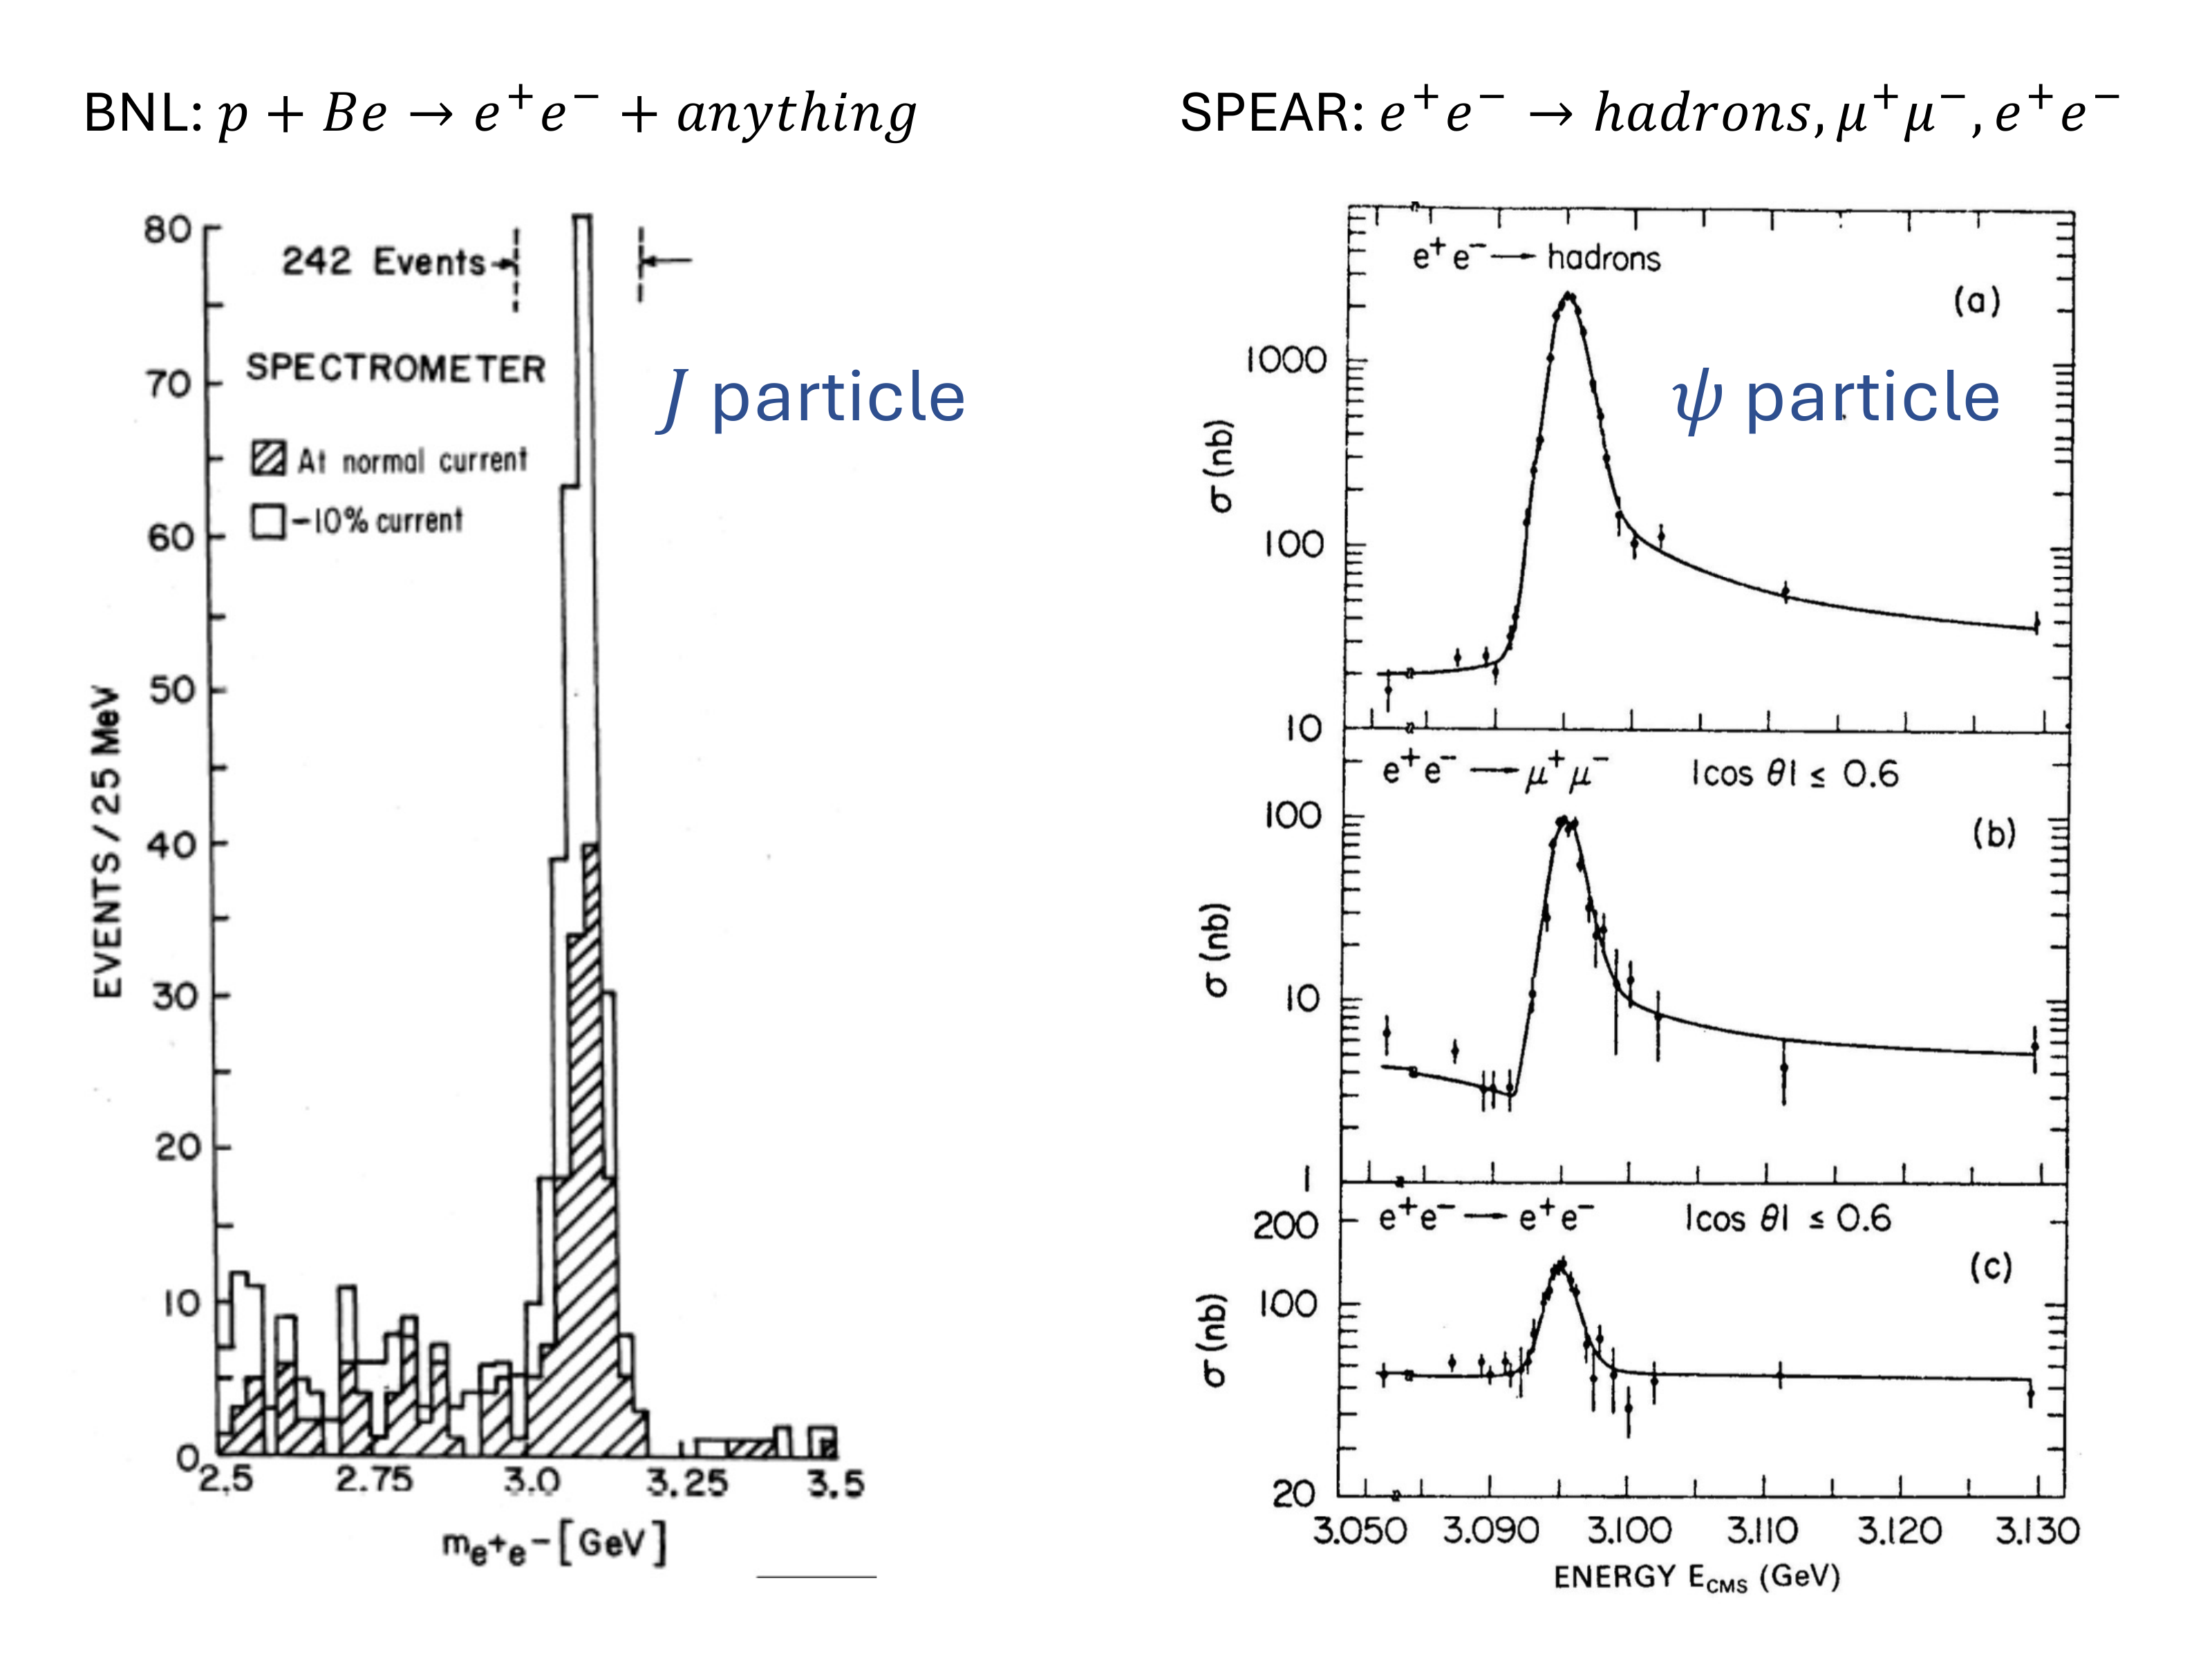
\includegraphics[width=0.95\textwidth]{Figures/jpsi_discovery.pdf}
%   \caption{The 1974 discovery of the $J/\psi$. Left: the heavy particle $J$ seen
%   by the BNL group in $p+\mathrm{Be}\to e^+e^-+X$. Right: the resonance $\psi$ seen
%   at SPEAR in three annihilation channels, fixing $J^{PC}=1^{--}$.}
%   \label{fig:jpsi-discovery}
% \end{figure}
% ------------------------------------------------------------

\FloatBarrier

% ============================================================
\subsection{Resonances}
\label{subsec:resonances}

An unstable particle is observed not as a sharp mass but as a peak of finite width in a
cross section or invariant-mass distribution. The shape of that peak follows directly from
the exponential character of radioactive decay. By Fermi's golden rule the transition rate
per unit time from an initial to a final state is
\begin{equation}
    T_{if} = 2\pi\,|\mathcal{M}|^2\,\rho(E_f),
    \label{eq:fermi-golden}
\end{equation}
where $\mathcal{M}$ is the transition matrix element and $\rho(E_f)$ the density of final
states. A sample of $N$ particles then obeys $\mathrm{d}N = -N\,T_{if}\,\mathrm{d}t$, whose
solution is the familiar exponential law $N = N_0\,e^{-t/\tau} = N_0\,e^{-\Gamma t}$, where
the mean lifetime $\tau$ and the total width $\Gamma$ are related by $\Gamma\tau = \hbar = 1$
in natural units.

A stable state of energy $E_0$ is described by a wavefunction $\psi(t) = \psi_0\,e^{-iE_0 t}$
whose probability density $|\psi(t)|^2 = |\psi_0|^2$ is constant in time. For an unstable
state the probability density must instead decay exponentially, which is achieved by giving
the energy a small imaginary part, so that
\begin{equation}
    \psi(t) = \psi(0)\,e^{-iE_0 t}\,e^{-t/2\tau},
    \qquad
    |\psi(t)|^2 = |\psi(0)|^2\,e^{-t/\tau}.
    \label{eq:decaying-state}
\end{equation}
The damped oscillation \eqref{eq:decaying-state} is no longer a single frequency: it
contains a spread of energies. The energy content is obtained from the Fourier transform,
\begin{equation}
    f(E) \sim \int_0^\infty \psi(0)\,e^{-i\left[(E_0 - E)t - i t/2\tau\right]}\,\mathrm{d}t
         \;=\; \frac{\psi(0)}{(E_0 - E) - i/(2\tau)} .
    \label{eq:fourier-resonance}
\end{equation}
The probability of finding the state with energy $E$ is then proportional to $|f(E)|^2$, and
with $\tau = 1/\Gamma$ this yields the \emph{non-relativistic Breit--Wigner distribution}
\begin{equation}
    |f(E)|^2 \;\propto\; \frac{(\Gamma/2)^2}{(E_0 - E)^2 + (\Gamma/2)^2},
    \label{eq:breit-wigner-intensity}
\end{equation}
a bell-shaped curve peaked at $E = E_0$ with a full width at half maximum equal to $\Gamma$
(Fig.~\ref{fig:breit-wigner}).

\begin{figure}[t]
    \centering
    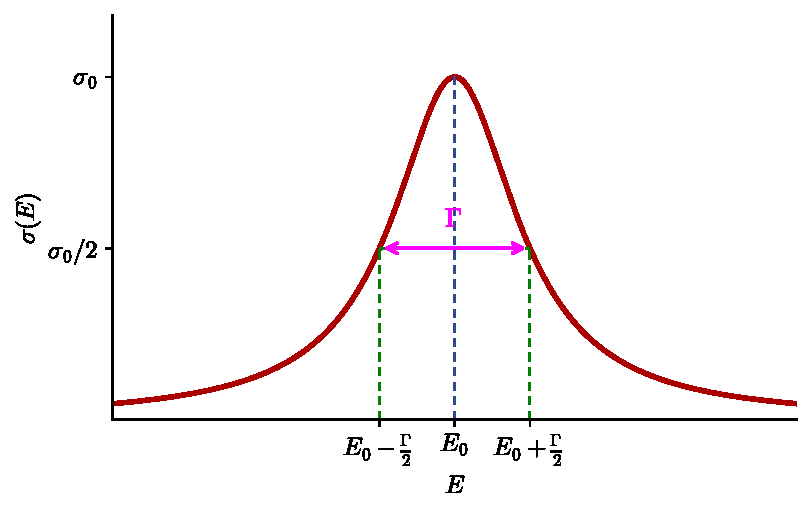
\includegraphics[width=0.62\textwidth]{Figures/breit_wigner.pdf}
    \caption{The non-relativistic Breit--Wigner line shape \eqref{eq:breit-wigner-intensity}.
    The peak sits at the resonance energy $E_0$ and the full width at half maximum equals the
    total width $\Gamma$.}
    \label{fig:breit-wigner}
\end{figure}

Resonances are most fundamentally described not by the intensity \eqref{eq:breit-wigner-intensity}
but by the underlying complex amplitude
\begin{equation}
    \mathrm{BW}(E) = \frac{\Gamma/2}{(E_0 - E) - i\,\Gamma/2}.
    \label{eq:breit-wigner-amplitude}
\end{equation}
Introducing the phase shift $\delta$ through $\cot\delta = 2(E_0 - E)/\Gamma$, the amplitude
takes the compact form
\begin{equation}
    f(E) = \frac{1}{\cot\delta - i} = e^{i\delta}\sin\delta,
    \label{eq:amplitude-phaseshift}
\end{equation}
which can equally be derived from the $S$-matrix. As the energy sweeps across the resonance,
the phase $\delta$ rises through $90^\circ$ at $E = E_0$, and the amplitude $f(E)$ traces a
circle in the complex plane---the \emph{Argand diagram}---reaching the top of the circle at
resonance. Real hadronic resonances are usually more complicated than this idealized
picture: overlapping resonances, several open decay channels, and energy-dependent widths
all distort the simple circle. The $\Delta(1232)$, seen as the $P_{33}$ partial wave in
$\pi N \to \pi N$ scattering, is the textbook example whose real and imaginary parts
approximate, but do not exactly reproduce, the ideal Breit--Wigner behaviour
\cite[Ch.~9]{Amsler2018}.

For a resonance formed in the collision of two particles with spins $s_1$ and $s_2$, the
energy dependence of the cross section combines the Breit--Wigner factor with the spin
multiplicities,
\begin{equation}
    \sigma(E) = \frac{4\pi}{k^2}\,
    \frac{\Gamma^2/4}{(E - E_R)^2 + \Gamma^2/4}\,
    \frac{2J + 1}{(2s_1 + 1)(2s_2 + 1)},
    \label{eq:resonance-cross-section}
\end{equation}
where $1/k = \lambda/2\pi = \hbar/p$ is the reduced de~Broglie wavelength of the colliding
particles in the centre-of-mass frame, $E$ the centre-of-mass energy, and $J$ the resonance
spin. Equation~\eqref{eq:resonance-cross-section} is the tool used in
Sect.~\ref{subsec:ozi-width} to extract the true $J/\psi$ width from the measured reaction
rate.

% ------------------------------------------------------------
% FIGURE SUGGESTION:
% Two-panel resonance figure complementing the generated Breit-Wigner plot.
% (left) Argand diagram: the amplitude T = BW(E) tracing the unitarity circle in
% the complex plane with the phase shift delta and the resonance point R at the top;
% (right) the measured P_33 (Delta(1232)) partial-wave amplitude in pi N -> pi N,
% real and imaginary parts versus W. Reproduce from the week 21 VL1 "Summary:
% Resonance" slide.
% \begin{figure}[t]
%   \centering
%   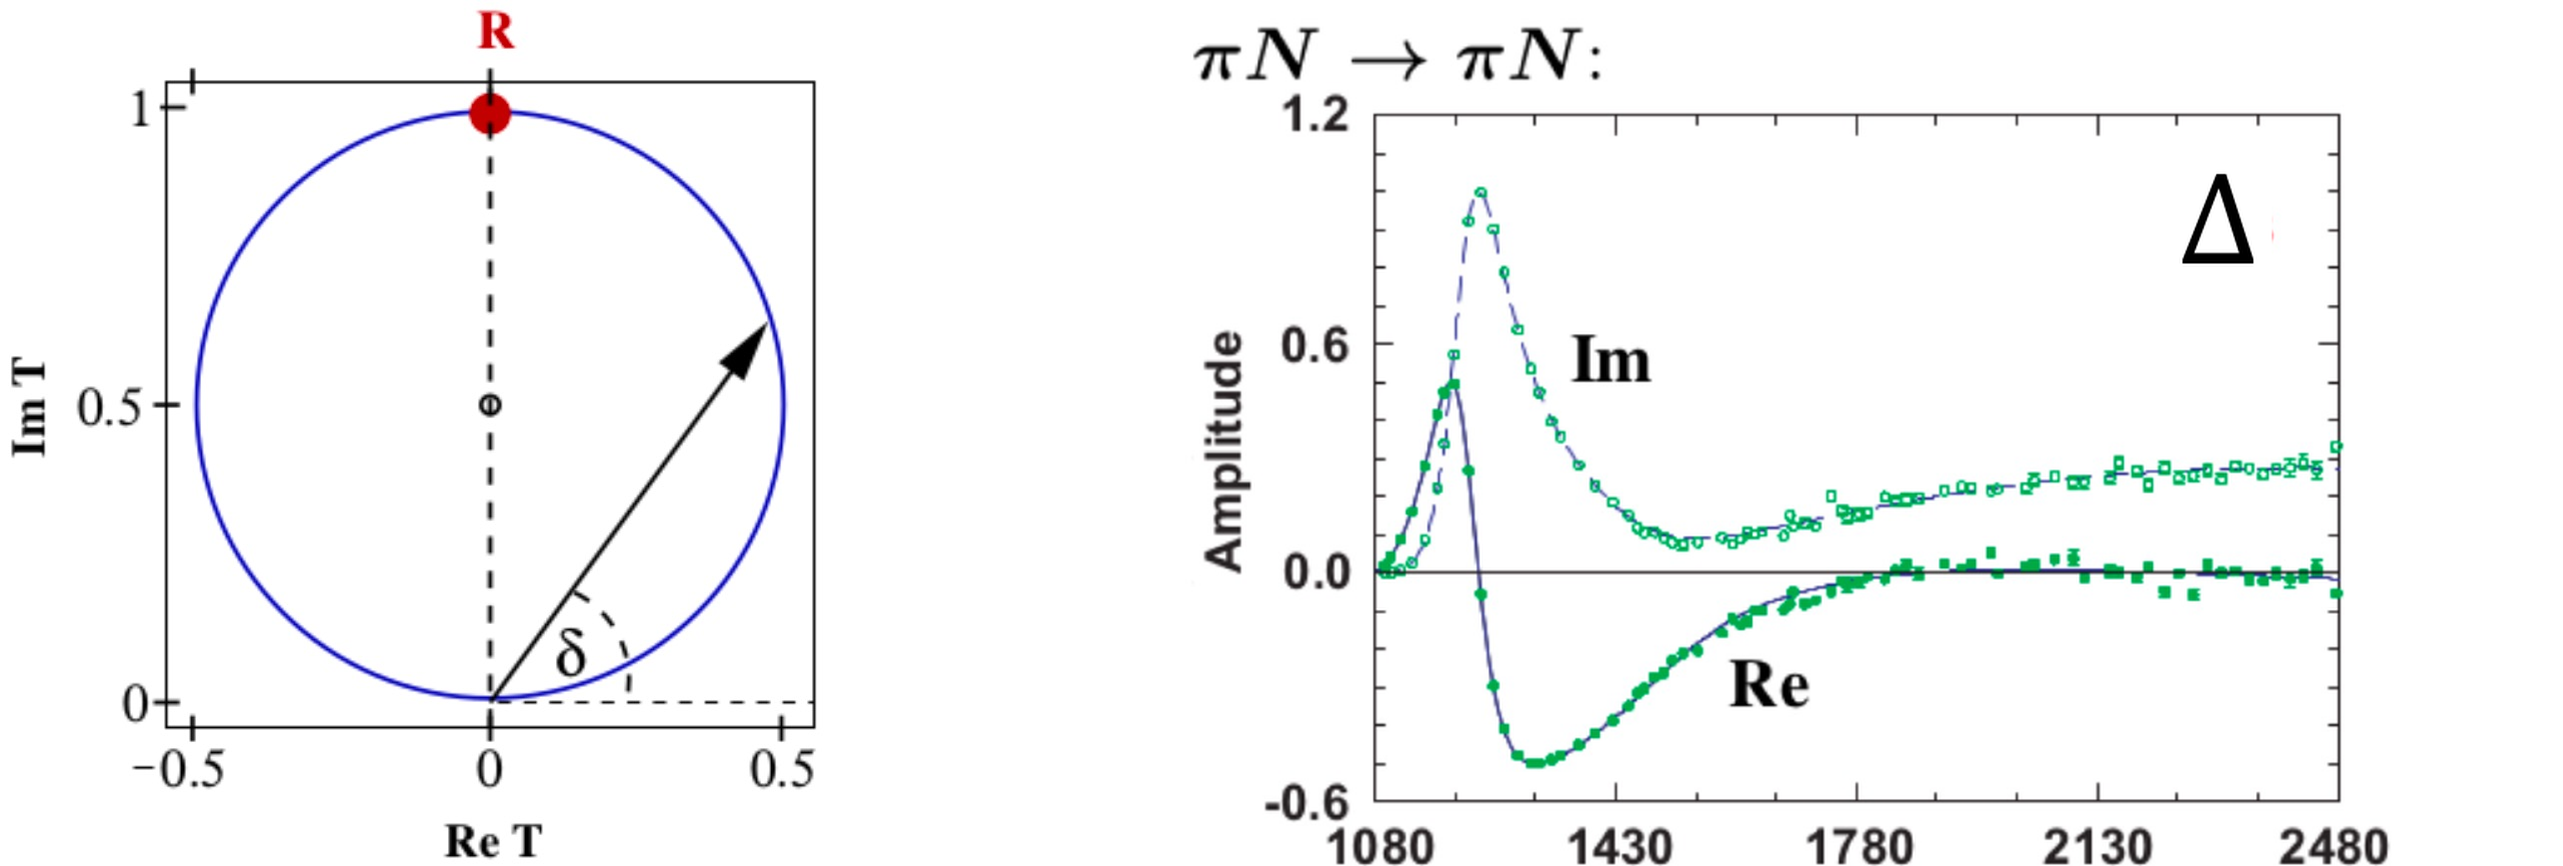
\includegraphics[width=0.9\textwidth]{Figures/argand_delta.pdf}
%   \caption{Left: Argand diagram of the resonant amplitude
%   \eqref{eq:amplitude-phaseshift}. Right: the $P_{33}$ ($\Delta(1232)$)
%   partial-wave amplitude in $\pi N$ scattering, illustrating departures from the
%   ideal circle.}
%   \label{fig:argand-delta}
% \end{figure}
% ------------------------------------------------------------

\FloatBarrier

% ============================================================
\subsection{The OZI rule and the width of the \texorpdfstring{$J/\psi$}{J/psi}}
\label{subsec:ozi-width}

The narrowness of the $J/\psi$ is explained by its position below the threshold for decay
into a pair of charmed mesons. The lightest charmed mesons have masses $m(D^\pm) =
1869\,\mathrm{MeV}$ and $m(D^0) = 1865\,\mathrm{MeV}$, so that the lowest open-charm
threshold lies near $2m(D) \approx 3.74\,\mathrm{GeV}$, well above the $J/\psi$ mass of
$3096.9\,\mathrm{MeV}$ \cite[Ch.~8]{Amsler2018}. The $J/\psi$ therefore cannot dissociate
into a $D\bar D$ pair, in which the initial $c$ and $\bar c$ are simply carried off into the
final mesons along connected quark lines. It is forced instead to decay through the
annihilation of the $c\bar c$ pair into light hadrons, a process governed by the
Okubo--Zweig--Iizuka (OZI) rule: decay amplitudes whose quark-line diagrams can be cut into
two disconnected pieces by severing only gluon lines are strongly suppressed.

The suppression can be quantified by counting gluons. In the decay $J/\psi \to 3\pi$ the
$c\bar c$ must annihilate completely, and no colour can be transmitted from the colour-singlet
$c\bar c$ state to the colour-singlet final hadrons except through a colourless combination
of at least two gluons. The quantum numbers tighten this further: an $n$-gluon system carries
charge conjugation $C = (-1)^n$, and matching the $J^{PC} = 1^{--}$ of the $J/\psi$ together
with colour neutrality requires at least three gluons, $n \geq 3$. Each of these gluons is
hard, since it must carry a momentum of order the charm mass, $q^2 \sim m_\psi^2$, where the
strong coupling is small. The annihilation rate is therefore proportional to $\alpha_s^6$
and is strongly suppressed, which accounts for the long lifetime and small width
\cite[Ch.~8]{Amsler2018}. By contrast, a heavier vector charmonium state lying above the
open-charm threshold, such as the $\psi(3770)$, can decay into $D\bar D$ through connected
quark lines requiring only a single soft gluon to create the additional light quark pair;
such states are correspondingly broad.

Because the apparent width of the $J/\psi$ is dominated by the experimental resolution, the
true width is far smaller than the observed peak and cannot be read off directly. It is
instead reconstructed from the total reaction rate and the leptonic branching ratio, using
the resonance cross section \eqref{eq:resonance-cross-section}. The integral of the
measured peak, combined with the fraction of decays into a known channel such as
$e^+e^-$ or $\mu^+\mu^-$, fixes the partial widths and hence the total width, yielding a
value of order $0.1\,\mathrm{MeV}$---two orders of magnitude smaller than the width of a
typical light-quark resonance such as the $\rho$ ($\Gamma \approx 150\,\mathrm{MeV}$ at
$m \approx 770\,\mathrm{MeV}$).

\FloatBarrier

% ============================================================
\subsection{The quark--antiquark potential and confinement}
\label{subsec:qq-potential}

The success of treating quarkonium as a non-relativistic bound state rests on a static
potential between the heavy quark and antiquark. The standard parametrization, the
\emph{Cornell potential}, combines a short-distance Coulomb-like term with a long-distance
linear term,
\begin{equation}
    V_{Q\bar Q}(r) = -\frac{4}{3}\,\frac{\alpha_s}{r} + k\,r,
    \label{eq:cornell-potential}
\end{equation}
with a representative strong coupling $\alpha_s = 0.3$ and string tension
$k = 1\,\mathrm{GeV\,fm^{-1}}$ \cite[Ch.~9]{Amsler2018}. The colour factor $4/3$ arises from
the $\mathrm{SU}(3)_c$ structure of one-gluon exchange between a colour and an anticolour
charge. At small separations the Coulomb term dominates and the potential resembles that of
electromagnetism, reflecting the asymptotic freedom of QCD; at large separations the linear
term dominates and grows without bound, the hallmark of confinement
(Fig.~\ref{fig:cornell-potential}).

\begin{figure}[t]
    \centering
    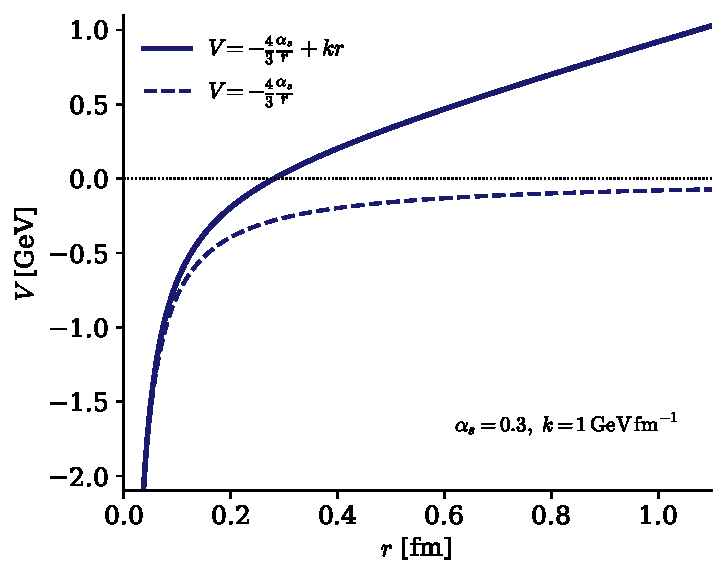
\includegraphics[width=0.6\textwidth]{Figures/cornell_potential.pdf}
    \caption{The Cornell quark--antiquark potential \eqref{eq:cornell-potential} for
    $\alpha_s = 0.3$ and $k = 1\,\mathrm{GeV\,fm^{-1}}$ (solid). The dashed curve shows the
    Coulomb-like term alone; the linear term produces the rising confining behaviour at
    large $r$.}
    \label{fig:cornell-potential}
\end{figure}

Spin-dependent corrections, suppressed by powers of the heavy-quark mass $m_Q$, generate the
fine and hyperfine structure of the spectrum. The spin--spin (contact) interaction,
\begin{equation}
    V_{SS} = \frac{8\pi\alpha_s}{9\,m_Q^2}\,\delta^3(\vec r)\,
    \vec S_Q \cdot \vec S_{\bar Q},
\end{equation}
splits states differing in total spin and acts only where the wavefunction overlaps at the
origin. The spin--orbit and tensor interactions,
\begin{align}
    V_{LS} &= \frac{1}{m_Q^2}\left(\frac{2\alpha_s}{r^3} - \frac{k}{2r}\right)
              \vec L \cdot \vec S, \\
    V_{T}  &= \frac{1}{m_Q^2}\,\frac{\alpha_s}{3r^3}
              \left(\frac{3\,(\vec S_Q\cdot\hat r)(\vec S_{\bar Q}\cdot\hat r)}{r^2}
              - \vec S_Q\cdot\vec S_{\bar Q}\right),
\end{align}
split the orbital multiplets and couple states of equal $J$ but different $L$ and $S$
\cite[Ch.~9]{Amsler2018}.

The linear term in \eqref{eq:cornell-potential} has a direct physical picture. Whereas the
electric field lines between two opposite charges spread out through space, giving the
familiar $1/r^2$ force, the colour field between a quark and an antiquark is squeezed into a
narrow flux tube, or string, of roughly constant energy per unit length. The force between
them is therefore approximately constant at large separation rather than falling off, so the
energy stored in the string rises linearly with distance. When enough energy is stored, it
becomes energetically favourable to create a new $q\bar q$ pair from the vacuum, the string
breaks, and two colour-singlet hadrons fly apart. This is why isolated colour charges are
never observed: pulling a quark out of a hadron produces more hadrons, not a free quark
\cite[Ch.~10]{Amsler2018}.

\FloatBarrier

% ============================================================
\subsection{Regge trajectories}
\label{subsec:regge}

Independent evidence for the linear confining potential comes from the systematics of the
light mesons. If the mass of a highly excited light meson resides almost entirely in the
energy of the gluonic string---the light quark masses being negligible---then a simple
rotating-string model predicts that the squared mass grows linearly with the total angular
momentum. The data bear this out strikingly: plotting $M^2$ against $J$ for the leading
$\rho/a$ and $\omega/f$ families produces straight lines, the \emph{Regge trajectories}
(Fig.~\ref{fig:regge}), with the $\rho(770)$, $f_2(1270)/a_2(1318)$,
$\omega_3(1670)/\rho_3(1700)$, $a_4(2020)/f_4(2050)$, $\rho_5(2350)$ and
$a_6(2450)/f_6(2510)$ falling on a common slope of order $1\,\mathrm{GeV^2}$ per unit of
spin \cite[Ch.~9]{Amsler2018}. The linearity of these trajectories is exactly what the
linear term of \eqref{eq:cornell-potential} implies for the large-$r$ behaviour of the
quark--antiquark system, tying the light-meson spectroscopy to the same confining dynamics
that governs the heavy quarkonia.

\begin{figure}[t]
    \centering
    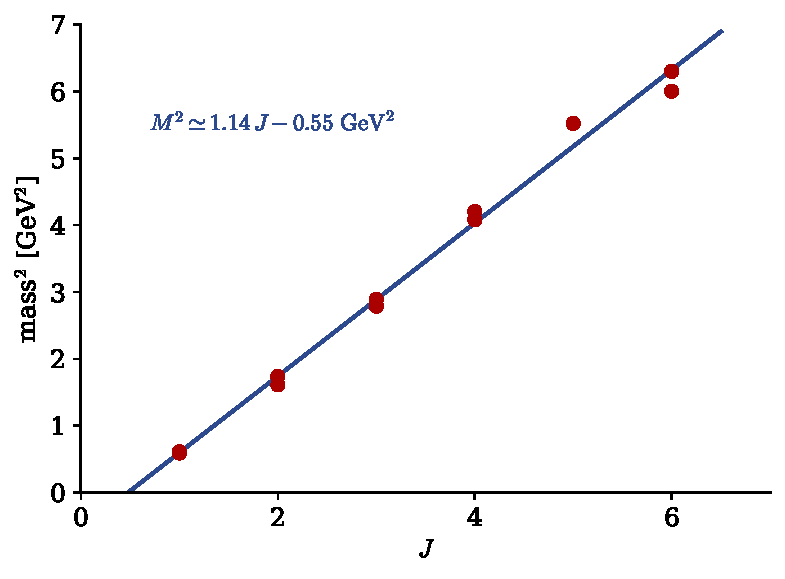
\includegraphics[width=0.62\textwidth]{Figures/regge_trajectory.pdf}
    \caption{Regge trajectory of the leading light mesons: the squared mass plotted against
    the total angular momentum $J$ falls on a straight line, consistent with a linear
    confining potential. The fitted slope is of order $1\,\mathrm{GeV^2}$ per unit spin.}
    \label{fig:regge}
\end{figure}

\FloatBarrier

% ============================================================
\subsection{The charmonium spectrum and potential models}
\label{subsec:charmonium-spectrum}

Because the charm quark is heavy, the $c\bar c$ system is non-relativistic and its spectrum
follows from solving the Schr\"odinger equation with the potential of
Sect.~\ref{subsec:qq-potential}. The states are labelled spectroscopically as
$n^{2S+1}L_J$, where $S$ is the total quark spin, $L$ the orbital angular momentum and $J$
the total angular momentum. A subtlety of nomenclature must be noted: for positronium the
principal quantum number is defined as $n = N + L + 1$, whereas for quarkonium the
convention $n = N + 1$ is used, where $N$ counts the radial nodes of the wavefunction
\cite[Ch.~9]{Amsler2018}.

The analogy with positronium is close in structure but vastly different in scale. Positronium
is bound by the electromagnetic interaction with coupling $\alpha = 1/137$ between particles
of mass $m_e = 0.511\,\mathrm{MeV}$, while charmonium is bound by the strong interaction with
$\alpha_s = 0.2$--$1$ between quarks of mass $m_c \approx 1600\,\mathrm{MeV}$. The
characteristic energy scale, which goes as $m\,\alpha^2$, is therefore larger for charmonium
by a factor of order $(m_c/m_e)(\alpha_s^2/\alpha^2) \sim 10^8$, so that positronium binding
energies measured in electron-volts correspond to charmonium splittings of hundreds of MeV.
The level ordering reflects the potential directly: because the Laplacian of the Cornell
potential is positive, $\nabla^2 V > 0$, the $P$ levels lie above the corresponding lower
$S$ levels, and indeed the $\chi_{cJ}(1P)$ states are found below the $\psi(2S)$
\cite[Ch.~9]{Amsler2018}. Potential models reproduce the measured charmonium spectrum well,
especially for the low-lying states.

% ------------------------------------------------------------
% FIGURE SUGGESTION:
% Side-by-side level schemes of charmonium and positronium drawn on a common
% spectroscopic grid (n^{2S+1}L_J), with the charmonium mass axis in GeV and the
% positronium binding-energy axis in eV, and the DD-bar threshold indicated on the
% charmonium side. Reproduce from the week 21 VL1 "Resulting spectrum" slide
% (charmonium vs positronium). A TikZ level diagram would be appropriate here.
% \begin{figure}[t]
%   \centering
%   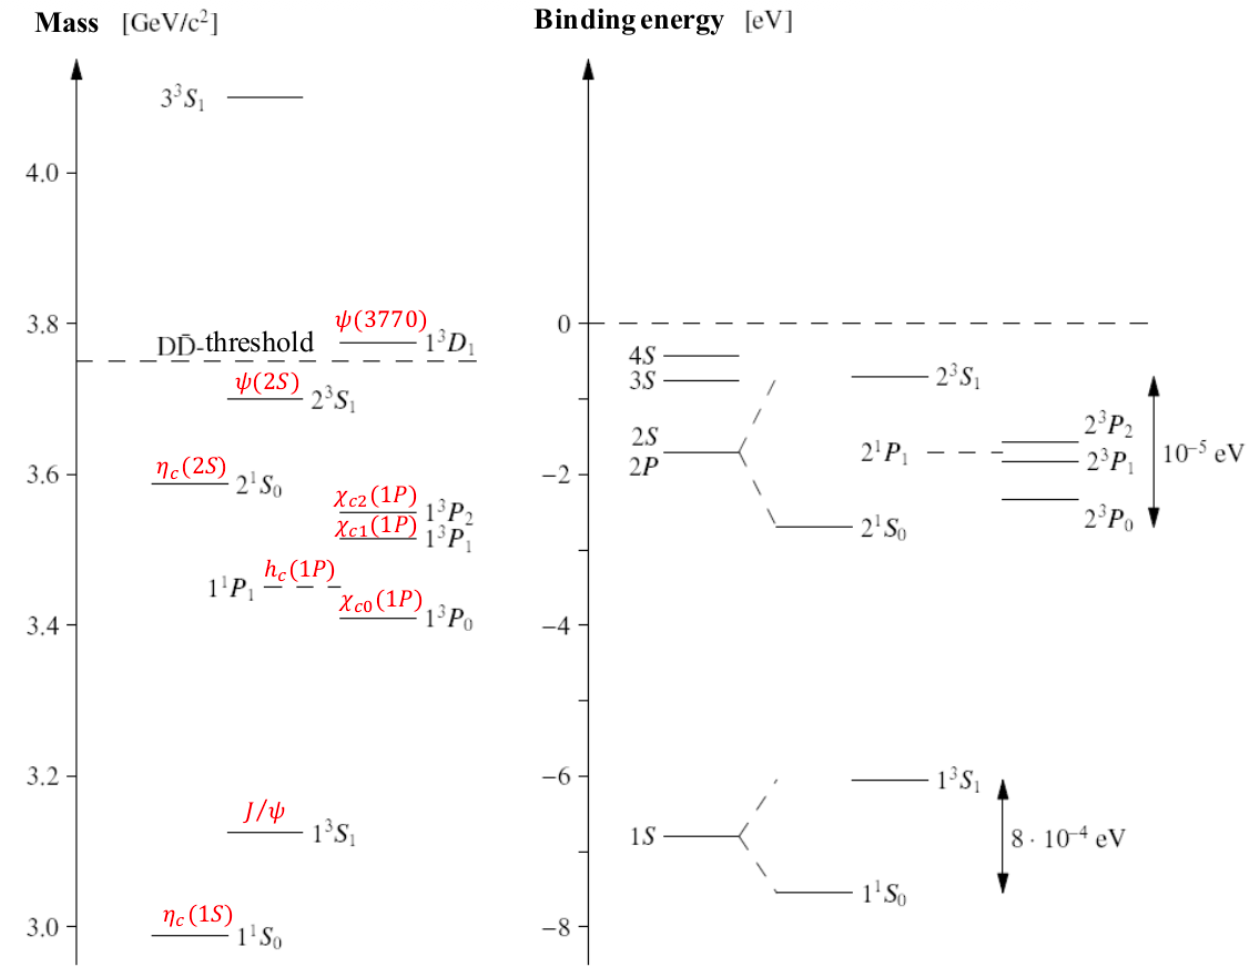
\includegraphics[width=0.85\textwidth]{Figures/charmonium_positronium.pdf}
%   \caption{The charmonium level scheme (left) compared with positronium (right),
%   showing the close structural analogy between an electromagnetically bound
%   $e^+e^-$ system and a strongly bound $c\bar c$ system.}
%   \label{fig:charmonium-positronium}
% \end{figure}
% ------------------------------------------------------------

\FloatBarrier

% ============================================================
\subsection{Probing charmonium: radiative decays and beam scans}
\label{subsec:charmonium-probes}

Only the $J^{PC} = 1^{--}$ states couple directly to the virtual photon and can therefore be
formed directly in $e^+e^-$ annihilation. The remaining charmonium levels are reached
indirectly, most cleanly through radiative transitions. The Crystal Ball experiment at SPEAR
mapped the spectrum by studying $e^+e^- \to \psi(2S) \to \gamma X$, in which the $\psi(2S)$
emits a photon and cascades to lower states \cite[Ch.~9]{Amsler2018}. The transitions obey
multipole selection rules. Electric dipole ($E1$) transitions have $\Delta L = 1$ and
$\Delta S = 0$ and connect the $1^{--}$ states to the $\chi_{cJ}$ ($J = 0, 1, 2$) states of
positive parity, so that the parity changes; magnetic dipole ($M1$) transitions have
$\Delta L = 0$ and $\Delta S = 1$ and connect to the $\eta_c$ states of $J = 0$ and negative
parity, leaving the parity unchanged. The measured masses of the principal states are
$\psi(1S) = 3096.9\,\mathrm{MeV}$, $\eta_c(1S) = 2983.9\,\mathrm{MeV}$,
$\psi(2S) = 3686.1\,\mathrm{MeV}$ and $\eta_c(2S) = 3637.7\,\mathrm{MeV}$. One early
radiative candidate, an $\eta_c'$ reported by Crystal Ball at $3592 \pm 5\,\mathrm{MeV}$,
was never confirmed and lay about $50\,\mathrm{MeV}$ too low for the potential models
\cite[Ch.~9]{Amsler2018}.

A limitation of the radiative method is that the spin-singlet $P$ state, the $h_c({}^1P_1)$,
cannot be reached from the $1^{--}$ levels by an allowed radiative transition. This state,
and precise widths in general, are accessible in proton--antiproton annihilation, exploited
by the E760 and E835 experiments at Fermilab. The advantage of the $p\bar p$ formation
technique is twofold. First, the antiproton beam energy can be tuned extremely precisely, so
that the resolution is set by the beam-momentum spread rather than by the calorimeter; E760
achieved a resolution of about $240\,\mathrm{keV}$, against the roughly $10\,\mathrm{MeV}$
typical of invariant-mass reconstruction in a detector. Second, this precision allows the
natural widths of the states to be resolved directly from a resonance scan. Scanning across
the $\chi_{c1}$ and $\chi_{c2}$ regions yielded
$\chi_{c1}(1P) = 3510.67 \pm 0.05\,\mathrm{MeV}$ and
$\chi_{c2}(1P) = 3556.17 \pm 0.07\,\mathrm{MeV}$, while the $\chi_{c0}$ was measured at a
mass of $3415.4\,\mathrm{MeV}$ with a width $\Gamma \approx 9.8\,\mathrm{MeV}$, and the
elusive $h_c(1P)$ was finally observed \cite[Ch.~9]{Amsler2018}. The same charmonium states
can also be produced in photoproduction, as pursued by the GlueX experiment through
$\gamma p \to \chi_{cJ}\,p$, which in addition offers a probe of the gluonic content of the
proton.

% ------------------------------------------------------------
% FIGURE SUGGESTION:
% Two related figures could be used here.
% (a) The Crystal Ball inclusive photon spectrum from e+e- -> psi(2S) -> gamma X,
%     with the radiative lines labelled, plus a level diagram with E1 (solid),
%     M1 (dashed), hadronic and 2-body EM transitions colour-coded.
% (b) The E760/E835 resonance scans across the chi_c1 and chi_c2 regions, cross
%     section versus sqrt(s), with the fitted Breit-Wigner curves.
% Reproduce from the week 21 VL1 "Charmonium Spectrum in Radiative Decays" and
% "Charmonium Spectrum in Beam Scans" slides.
% \begin{figure}[t]
%   \centering
%   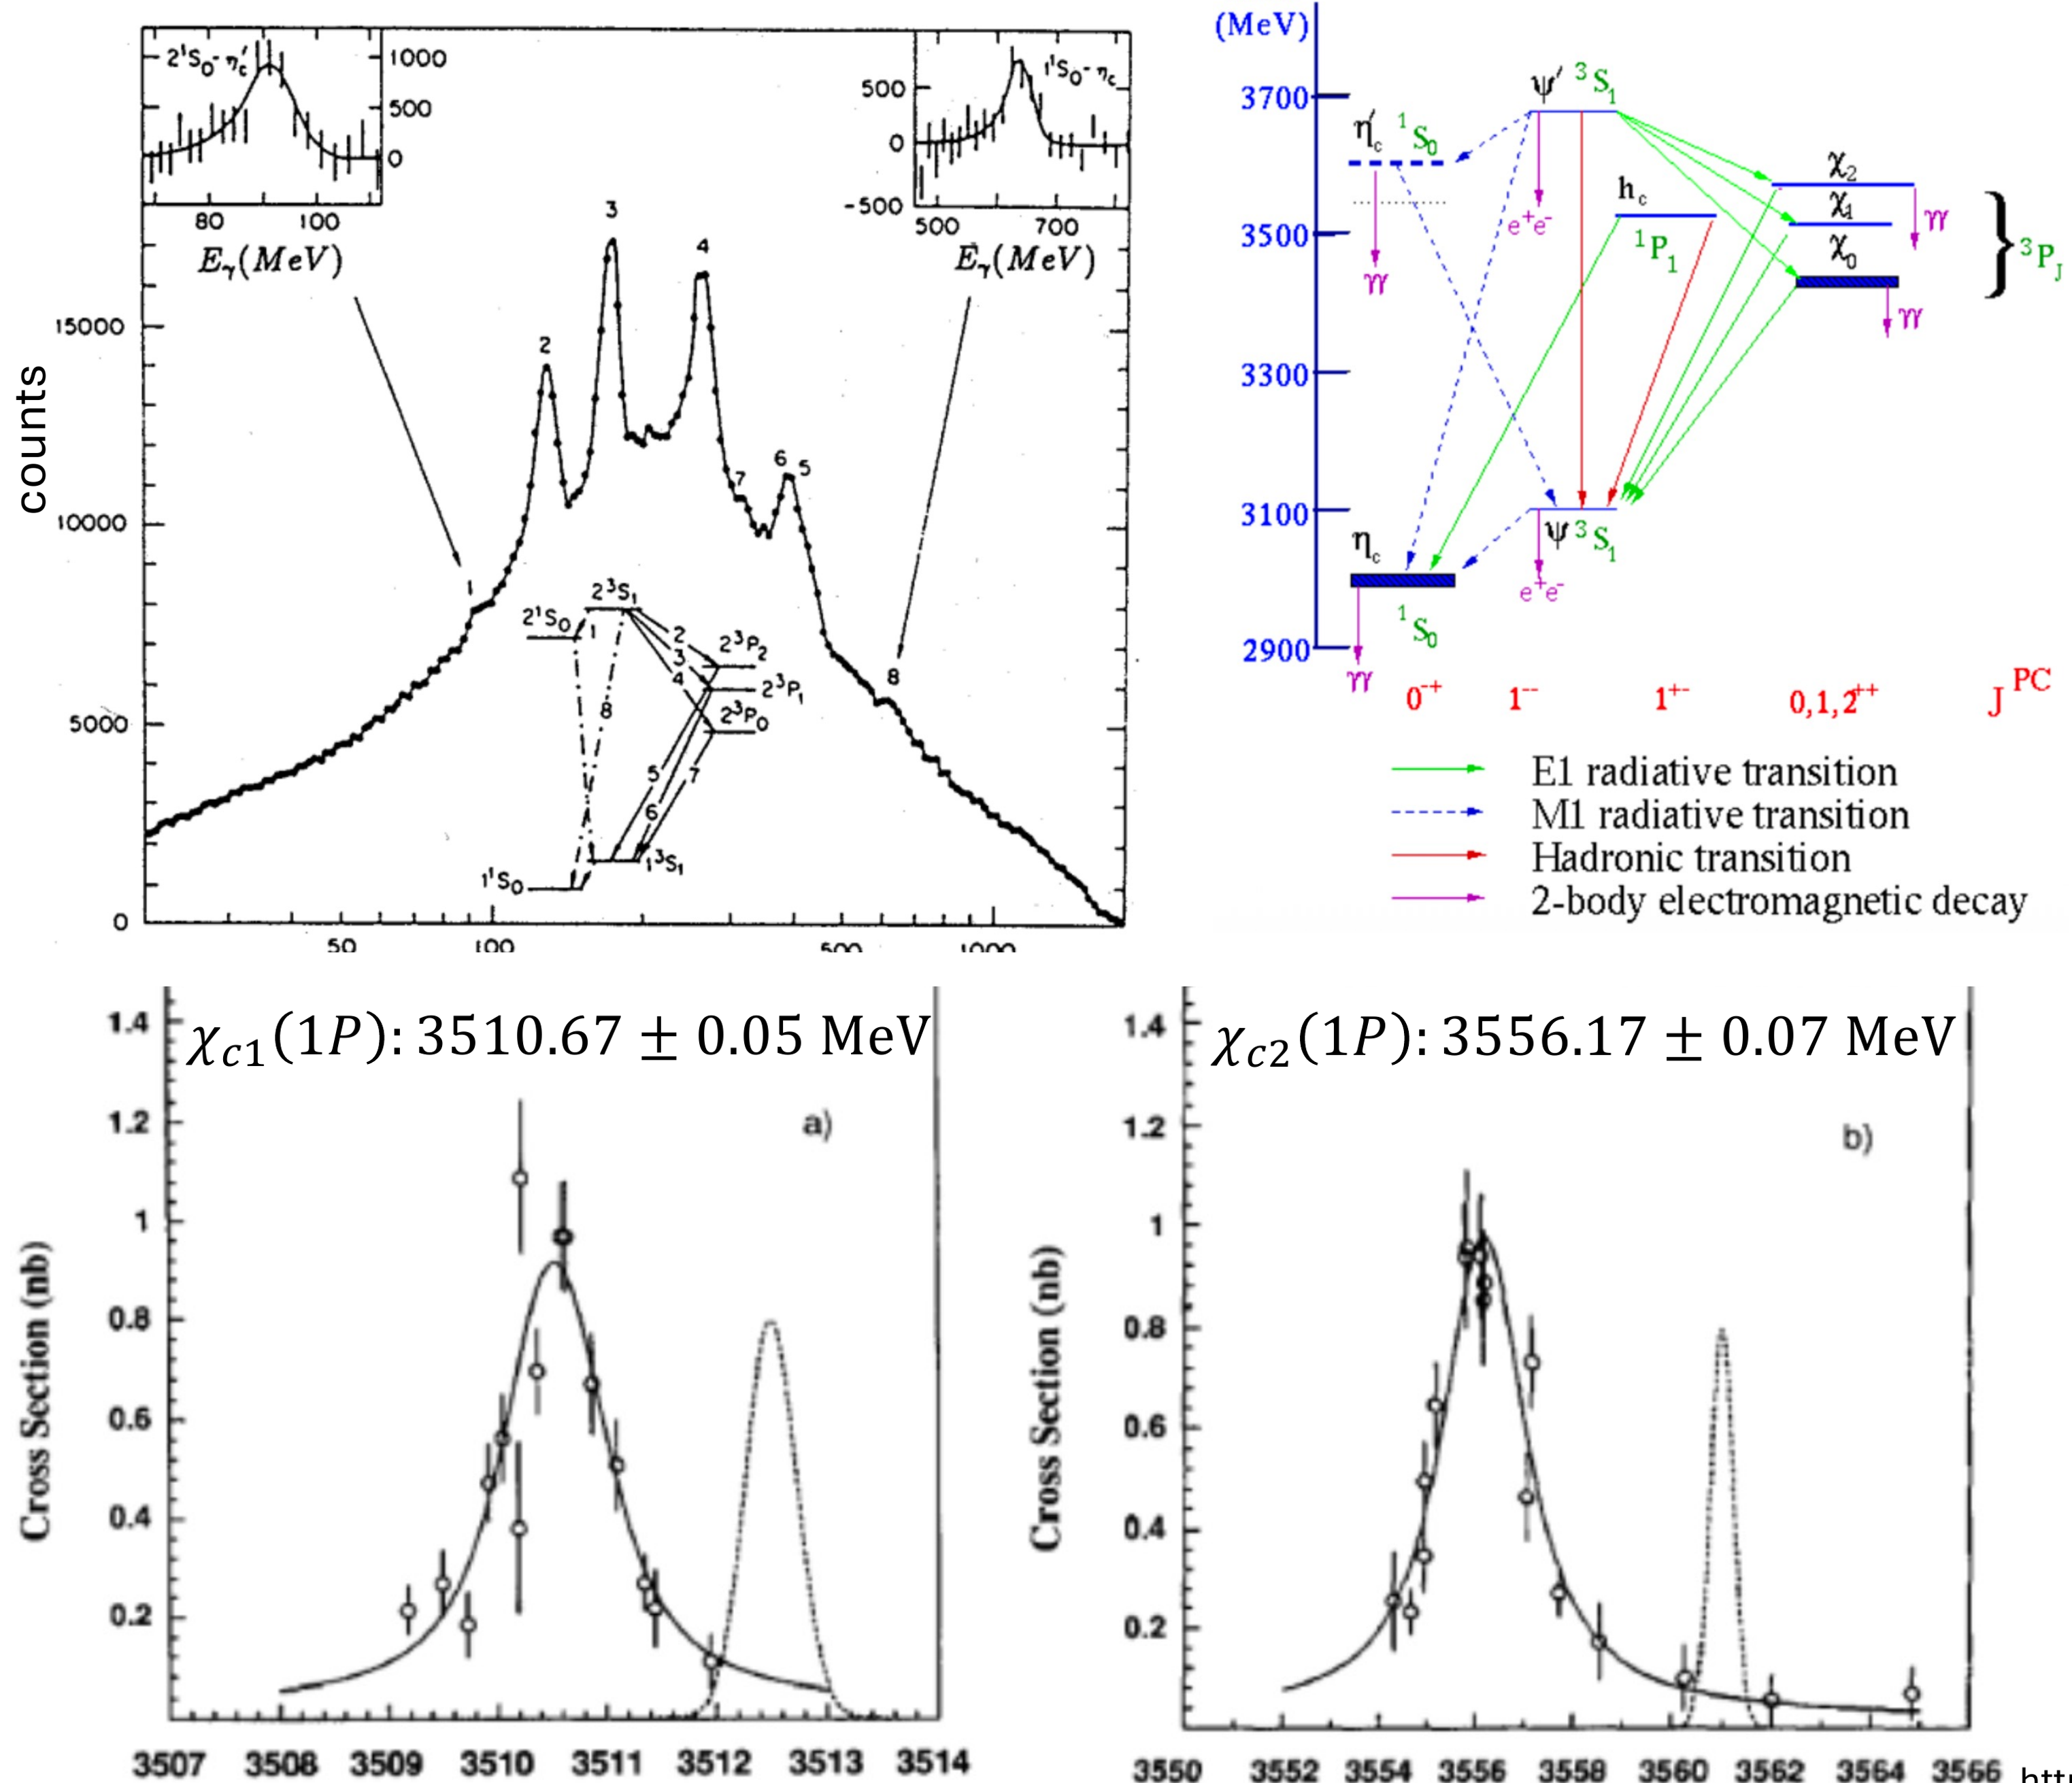
\includegraphics[width=0.9\textwidth]{Figures/charmonium_radiative_scan.pdf}
%   \caption{Probing the charmonium spectrum. Left: radiative photon spectrum from
%   $\psi(2S)\to\gamma X$ (Crystal Ball). Right: $p\bar p$ formation scans of the
%   $\chi_{c1}(1P)$ and $\chi_{c2}(1P)$ (E760/E835), whose narrow widths are
%   resolved by the precise beam momentum.}
%   \label{fig:charmonium-radiative-scan}
% \end{figure}
% ------------------------------------------------------------

\FloatBarrier

% ============================================================
\subsection{Bottomonium and the comparison of quarkonia}
\label{subsec:bottomonium}

Replacing the charm quark by the still heavier bottom quark produces bottomonium, the
$b\bar b$ system, observed in $e^+e^-$ annihilation at centre-of-mass energies near
$10\,\mathrm{GeV}$. Just as for charmonium, the lowest vector states---the $\Upsilon(1S)$,
$\Upsilon(2S)$ and $\Upsilon(3S)$---appear as very narrow resonances, for the same reason:
they lie below the threshold for decay into a pair of bottom mesons, which opens at
$10.558\,\mathrm{GeV}$. States above this threshold, such as the $\Upsilon(4S)$, decay
readily into $B\bar B$ and are broad. The resulting $b\bar b$ spectrum is closely analogous
to that of $c\bar c$ \cite[Ch.~9]{Amsler2018}.

A comparison of positronium, charmonium and bottomonium on a common spectroscopic footing
reveals both the universality and the limits of the potential picture. The lower-lying
levels have a very similar structure across all three systems, confirming that the same
functional form of the potential governs them. For the higher-lying levels, however, the
spacing decreases less rapidly than the $1/n^2$ law of a pure Coulomb potential, a direct
consequence of the linear confining term, and the $P$ states are positioned differently
relative to the $2S$ states in each system. The spin-singlet $h_b$ states, like their
charmonium counterpart, are not reached by radiative transitions and were instead first
observed by the Belle collaboration in $e^+e^- \to \Upsilon(5S) \to \pi^+\pi^- +
\text{hadrons}$, yielding the first observation of the $h_b(1P)$ and $h_b(2P)$
\cite[Ch.~9]{Amsler2018}. The $\psi$ and $\Upsilon$ families are now routinely used as
production engines for hadron spectroscopy at $e^+e^-$ colliders, with many discoveries
driven by data taken directly on resonance.

% ------------------------------------------------------------
% FIGURE SUGGESTION:
% Two figures are appropriate.
% (a) The R-ratio / e+e- cross section in the bottomonium region (sqrt(s) ~ 9.4-11.2
%     GeV) showing the narrow Upsilon(1S,2S,3S) peaks below, and the broad
%     Upsilon(4S) at, the B-meson threshold.
% (b) A three-panel comparison of the positronium, charmonium and bottomonium level
%     schemes on a shared n^{2S+1}L_J grid, illustrating the similar low-lying
%     structure and the differing high-lying spacings.
% Reproduce from the week 21 VL1 "R-plot revisited - Bottomonium" and "Comparison of
% e+e- vs cc vs bb" slides.
% \begin{figure}[t]
%   \centering
%   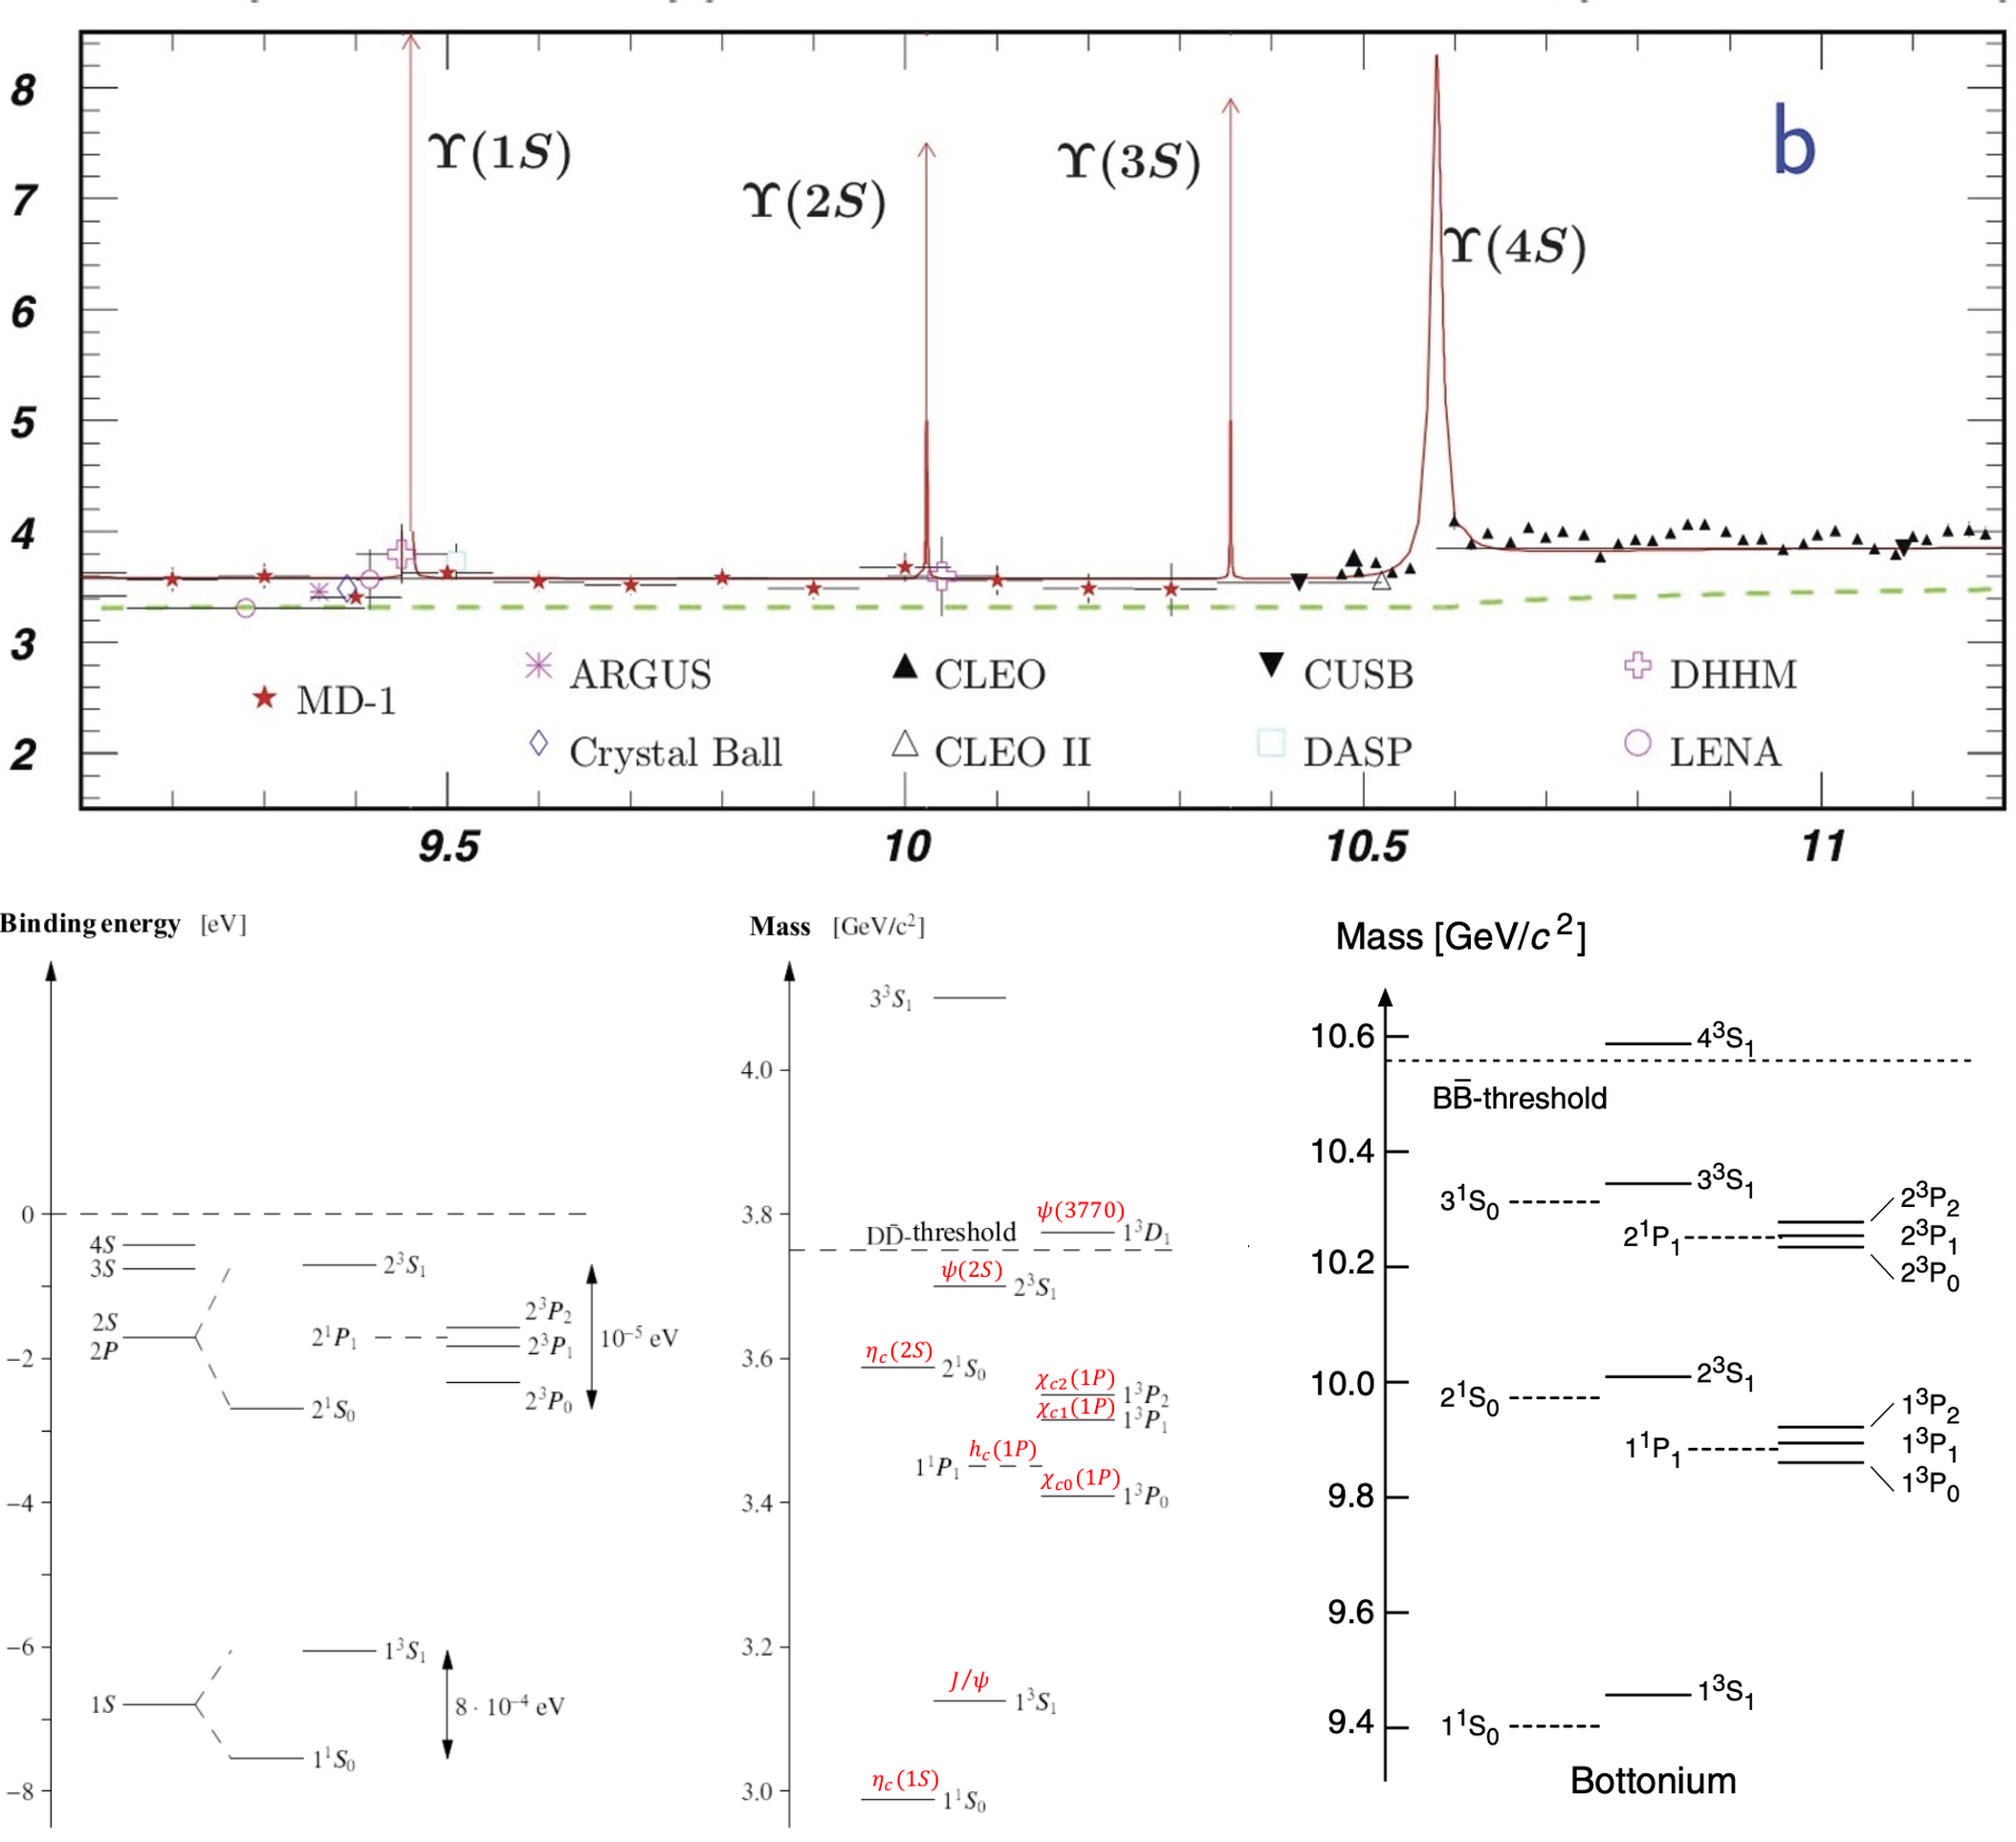
\includegraphics[width=0.95\textwidth]{Figures/bottomonium_comparison.pdf}
%   \caption{Left: the $b\bar b$ resonances in $e^+e^-$ annihilation, narrow below
%   the $B\bar B$ threshold at $10.558\,\mathrm{GeV}$ and broad above it. Right:
%   positronium, charmonium and bottomonium level schemes compared on a common grid.}
%   \label{fig:bottomonium-comparison}
% \end{figure}
% ------------------------------------------------------------

\FloatBarrier

% ============================================================
\subsection{Exotic States}
\label{subsec:exotic-states}

For the low-lying states the charmonium spectrum is a triumph of the potential model, but at
higher energies, near and above the open-charm threshold, the picture becomes far more
intricate. Since 2003 more than forty new states have been discovered that are difficult or
impossible to accommodate within the simple $q\bar q$ scheme, and several are manifestly
four-quark objects. Collectively known as the $XYZ$ states, they have driven a revival of
hadron spectroscopy, and the interpretation of most of them remains ambiguous
\cite[Ch.~16]{Amsler2018}.

The prototype is the $X(3872)$, discovered by the Belle collaboration in 2003 in the decay
$B^+ \to K^+ X$ with $X \to J/\psi\,\pi^+\pi^-$, and since confirmed by many experiments in
many modes. Its mass, $m(X) = 3871.64 \pm 0.06\,\mathrm{MeV}$, lies extraordinarily close to
the $D^0\bar D^{*0}$ threshold of $3871.68 \pm 0.07\,\mathrm{MeV}$, and its width is
remarkably small, $\Gamma = 1.19 \pm 0.21\,\mathrm{MeV}$. The dipion substructure of the
decay is dominated by the $\rho$, so that the process proceeds as $X(3872) \to J/\psi\,\rho
\to J/\psi\,\pi^+\pi^-$, which violates isospin. In 2013 LHCb established the quantum numbers
as $J^{PC} = 1^{++}$, the same as those of the charmonium state $\chi_{c1}(2{}^3P_1)$
\cite[Ch.~16]{Amsler2018}.

These observations support several competing interpretations, none of which is fully
satisfactory on its own. The $X(3872)$ might be the missing $\chi_{c1}(2P)$ charmonium state,
but that level is predicted about $50\,\mathrm{MeV}$ higher and with a much larger width, and
its expected dominant decay to $\gamma\chi_{c1}(1P)$ is not observed. Its proximity to the
$D^0\bar D^{*0}$ threshold and its large coupling to that channel suggest instead a weakly
bound $D\bar D^{*}$ ``molecule,'' analogous to the deuteron. Alternatively, its sizeable
prompt production in $pp$ collisions points toward a compact tetraquark. The most likely
resolution is that the physical state mixes more than one of these configurations
\cite[Ch.~16]{Amsler2018}. These possibilities motivate three generic pictures of multiquark
states: the compact \emph{tetraquark}, a colour-bound object formed from a $Qq$ diquark and a
$\bar Q\bar q$ antidiquark; the \emph{hadro-quarkonium} state, a compact $Q\bar Q$ core
surrounded by light quarks; and the \emph{hadronic molecule}, an extended object made of a
$\bar Q q$ meson loosely bound to a $Q\bar q$ meson.

The exotic zoo extends well beyond the $X$ states. The $Y$ states are vector ($1^{--}$)
resonances; the $Y(4260)$, found by BaBar in $e^+e^- \to \gamma_{\mathrm{ISR}}\,J/\psi\,
\pi^+\pi^-$, couples strongly to $J/\psi\,\pi^+\pi^-$ but only weakly to open charm, and is
supernumerary among the expected $1^{--}$ charmonia. The $Z$ states are electrically charged:
studying the $Y(4260)$ in $e^+e^-$ collisions, BESIII found a peak in the $\pi^\pm J/\psi$
subsystem, the $Z_c(3900)$. Since the $J/\psi$ already implies a minimal $c\bar c$ content, a
\emph{charged} state decaying to it cannot be an ordinary $c\bar c$ meson and must contain at
least four quarks. The same phenomenon recurs in bottomonium: the Belle collaboration,
studying $e^+e^- \to \Upsilon(5S) \to \pi^+\pi^-\Upsilon(nS)$ for $n = 1, 2, 3$, found the
charged $Z_b(10610)$ and $Z_b(10650)$ in the $\pi^\pm\Upsilon(nS)$ subsystem
\cite[Ch.~16]{Amsler2018}. Under the modern naming convention these families are organized as
the $X$ states (reassigned to $\chi$-type charmonia, e.g.\ $X(3872) \to \chi_{c1}(3872)$),
the $Y$ states ($1^{--}$, reassigned to $\psi$-type, e.g.\ $Y(4260) \to \psi(4230)$), and the
charged $Z$ states (reassigned as tetraquark-type $T$ states, e.g.\ $Z_c(3900) \to
T_{c\bar c1}(3900)$).

Still heavier and more exotic configurations have since emerged. Double-$J/\psi$ production,
reported by LHCb in 2020 and measured with higher statistics by CMS in 2024, reveals
structures in the $J/\psi\,J/\psi \to 4\mu$ invariant-mass spectrum that have been
interpreted as fully charmed tetraquarks $T_{c\bar c c\bar c}(6600)$,
$T_{c\bar c c\bar c}(6900)$ and $T_{c\bar c c\bar c}(7100)$. A qualitatively new type of
exotic appeared with the LHCb observation, in $pp$ collisions, of the $T_{cc}^+$ in the
$D^0 D^0 \pi^+$ invariant-mass spectrum. Its minimal quark content is $cc\bar u\bar d$,
containing two charm quarks of the same flavour, and it lies just below the $D^{*+}D^0$
threshold, $m_{T_{cc}^+} - (m_{D^{*+}} + m_{D^0}) = -273\,\mathrm{keV}$
\cite[Ch.~16]{Amsler2018}. Exotic states of these kinds were anticipated on general grounds
once QCD allowed colour-singlet combinations beyond $q\bar q$ and $qqq$; the difficulty is
that finding them has proved far easier than understanding them, and disentangling the
compact-tetraquark, hadro-quarkonium and molecular interpretations will require both more
data and improved theory.

% ------------------------------------------------------------
% FIGURE SUGGESTION:
% Several figures could illustrate this subsection.
% (a) The XYZ charmonium-region spectrum: invariant mass versus J^{PC}, with the
%     established cc states in one colour and the exotic X, Y, Z (and T) states
%     tagged, indicating which sit near open-charm thresholds. Reproduce from the
%     week 21 VL2 "The XYZ spectrum" slide (right panel).
% (b) The X(3872) signal: the J/psi pi+pi- invariant mass from Belle in
%     B+ -> K+ J/psi pi+pi-, and the mass measurements relative to the D0 D-bar*0
%     threshold. Reproduce from the week 21 VL1 "A surprise at higher energies:
%     X(3872)" and "X(3872): Observations" slides.
% (c) The three multiquark cartoons (compact tetraquark, hadro-quarkonium, hadronic
%     molecule). Reproduce from the week 21 VL2 "Summary: Multiquark Exotics" slide;
%     a TikZ schematic would be appropriate.
% (d) The CMS di-J/psi spectrum showing the T_cccc(6600/6900/7100), and the LHCb
%     T_cc+ peak in D0 D0 pi+ near threshold.
% \begin{figure}[t]
%   \centering
%   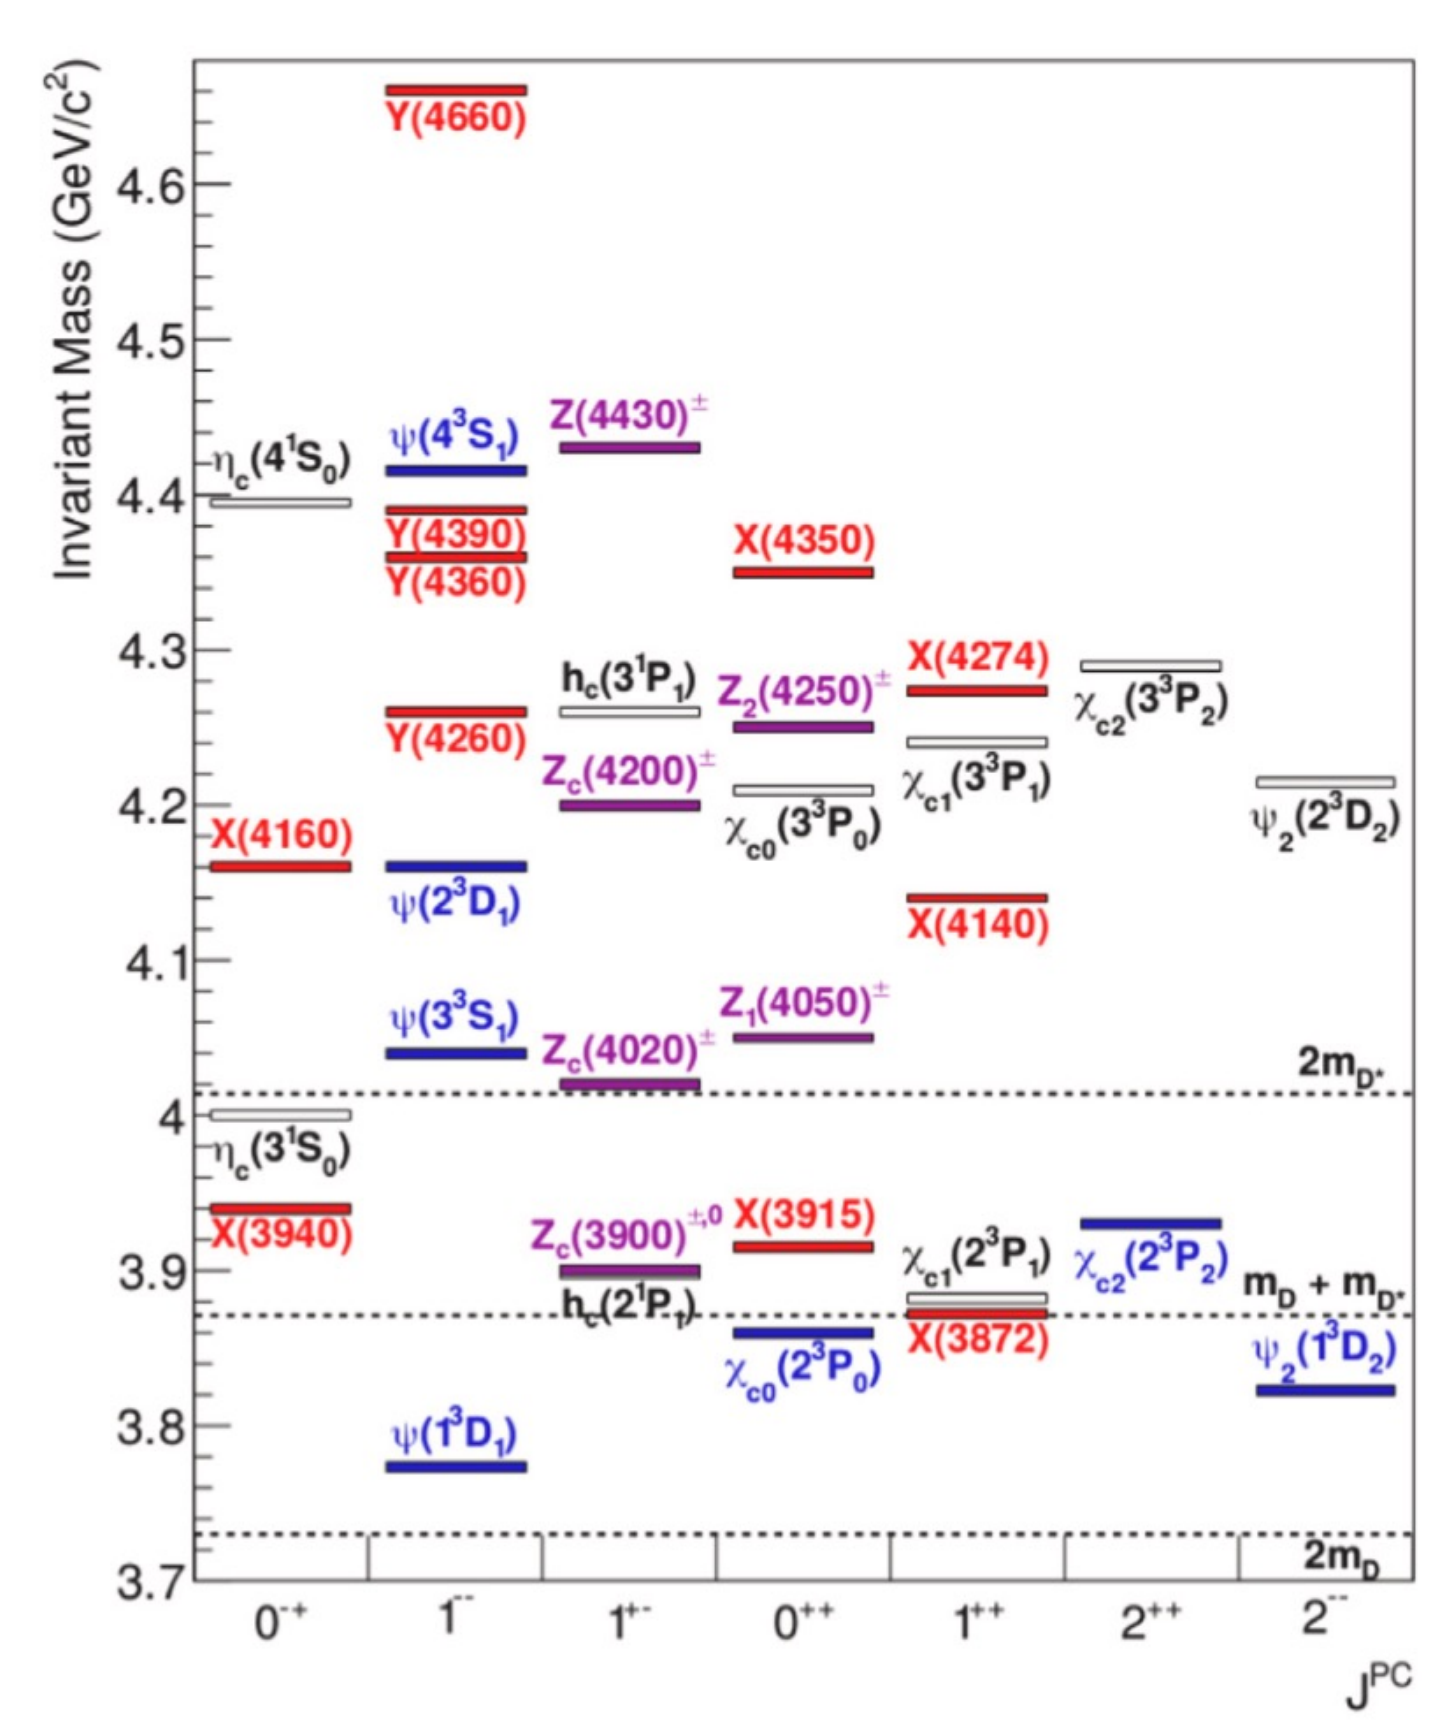
\includegraphics[width=0.95\textwidth]{Figures/xyz_spectrum.pdf}
%   \caption{The $XYZ$ states populating the charmonium region. Established $c\bar c$
%   levels are shown alongside the exotic candidates, many of which cluster near
%   open-charm thresholds.}
%   \label{fig:xyz-spectrum}
% \end{figure}
% ------------------------------------------------------------

\FloatBarrier